\chapter{Análisis del problema}

Como hemos comentado en el anterior capítulo, la principal competencia actual está 
bastante anticuada, especialmente en el ámbito de los memes.
\\\\
Para convertir este proyecto en algo viable y competitivo, deberemos asegurarnos de que
el usuario tenga una experiencia fluída, en contraposición con el resto de editores.
\\\\
Una de las principales carácterísticas que debe tener es poder cargar, editar y subir sin
necesidad de descargar nada en ningún momento.
\\\\
Hemos planteado que el editor esté formado por las siguientes partes:

\begin{figure}[!h]
    \centering
    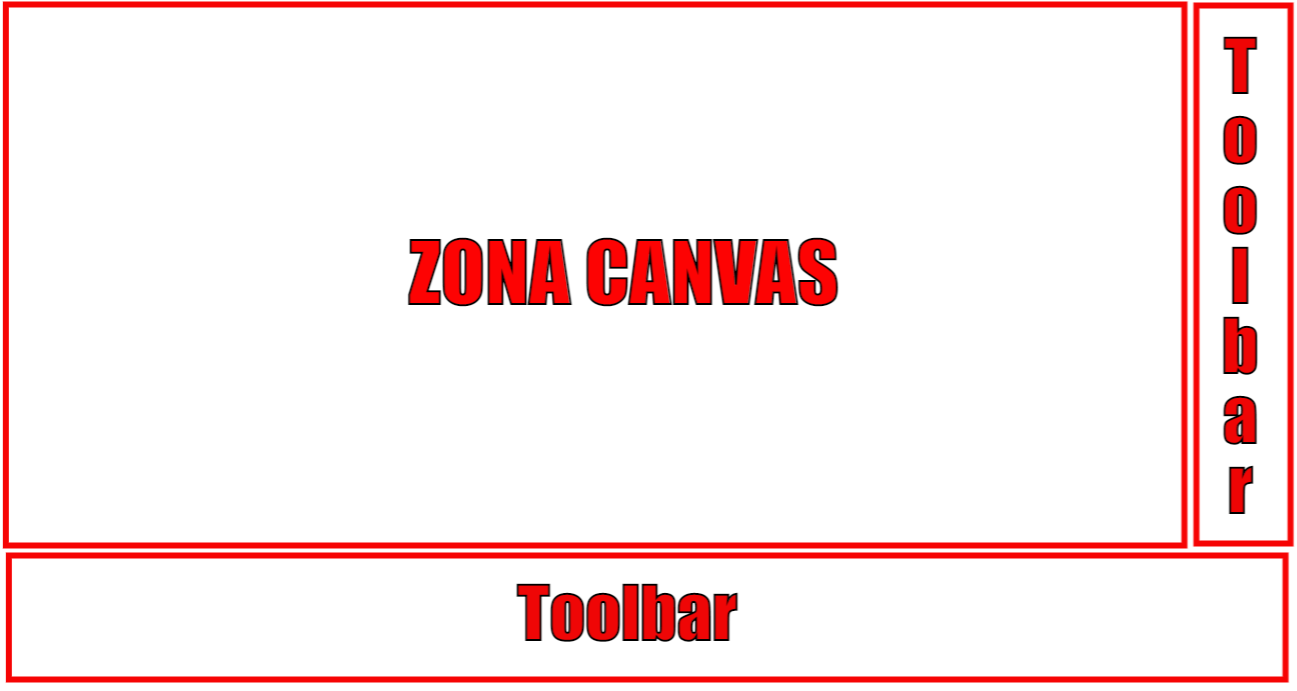
\includegraphics[scale=0.30]{img/ESQUEMA_ABSTRACTO.png}
    \caption{Esquema de las partes que debería tener el editor}
\end{figure}